\documentclass[conference,onecolumn,11pt]{IEEEtran}

\usepackage[utf8]{inputenc}
\usepackage[T1]{fontenc}
\usepackage{amsmath,amssymb,amsfonts}
\usepackage{graphicx}
\usepackage{booktabs}
\usepackage{hyperref}
\usepackage{xcolor}
\usepackage{braket}
\usepackage{multirow}
\usepackage[caption=false]{subfig}

\graphicspath{{./}{results/plots/}}

\title{Evaluating Quantum Data Encoding Strategies and Gradient Trainability for NLP Sentiment Analysis}

\author{\IEEEauthorblockN{Kadir G\"{o}ksel G\"{u}nd\"{u}z}
\IEEEauthorblockA{Energy Science and Technology\\
Istanbul Technical University (\.{I}T\"{U})\\
Istanbul, Turkey}}

\begin{document}

\maketitle

% ===================================================================
% ABSTRACT
% ===================================================================
\begin{abstract}
Selecting an appropriate data encoding strategy is a critical yet under-explored design decision for variational quantum circuits in natural language processing. We systematically compare four quantum encoding strategies --- Angle, Dense Angle, IQP, and Data Re-uploading --- on binary sentiment classification using IMDb and SST-2 benchmarks. Our pipeline embeds text via a frozen DistilBERT encoder, reduces dimensionality through PCA (768 to 8 features), and maps features into parameterized quantum circuits trained end-to-end with PyTorch-native statevector simulation. We find that: (1)~encoding ranking is dataset-agnostic, with Angle encoding consistently achieving the highest accuracy ($70.1\% \pm 1.1\%$ on IMDb, $76.4\%$ on SST-2); (2)~gradient variance measured at initialization correlates with but does not determine final accuracy --- high variance facilitates optimization yet does not guarantee performance, while compact architectures (Dense Angle) can achieve strong results despite low variance; (3)~sigmoid preprocessing of PCA features yields a $+17$-point accuracy improvement, highlighting the importance of input-domain alignment; and (4)~validation on IBM quantum hardware (ibm\_fez, 156 qubits) confirms 100\% simulator--QPU prediction agreement across all four encodings on a balanced test set (5 label-0~+~5 label-1), with zero T1 relaxation bias detected. Our results provide a practical decision framework for encoding selection in NISQ-era quantum NLP.
\end{abstract}

\begin{IEEEkeywords}
variational quantum circuits, data encoding, natural language processing, sentiment analysis, barren plateaus, NISQ
\end{IEEEkeywords}

% ===================================================================
% 1. INTRODUCTION
% ===================================================================
\section{Introduction}

Variational quantum circuits (VQCs) have emerged as a leading paradigm for near-term quantum machine learning, offering parameterized ans\"{a}tze trainable via classical optimization~\cite{cerezo2021vqa,bharti2022nisq}. A fundamental yet often overlooked design choice in VQCs is the \emph{data encoding strategy} --- the method by which classical features are mapped onto quantum states. While extensive work has studied ansatz architecture and training dynamics, the impact of encoding selection on downstream task performance remains poorly characterized, particularly for natural language processing (NLP) tasks.

Recent work in quantum NLP has explored various hybrid architectures combining classical language models with quantum circuits~\cite{tomal2025,sasquatch,setfit_pqc,hyqut,gqhan}. However, these studies typically adopt a single encoding strategy without systematic comparison across alternatives. This gap is significant because the encoding determines the structure of the quantum feature space, directly affecting both the expressibility of the model and its trainability.

The barren plateau phenomenon --- exponential vanishing of gradients with circuit depth or width --- has been identified as a critical obstacle for VQC training~\cite{mcclean2018barren,cerezo2021cost}. While barren plateaus are typically studied in the context of ansatz design, the encoding strategy also influences gradient landscape properties. An encoding that maps data into a region of the Hilbert space where gradients vanish effectively renders the circuit untrainable regardless of the ansatz quality.

In this work, we make the following contributions:

\begin{enumerate}
\item \textbf{Systematic encoding comparison for NLP.} We implement and compare four encoding strategies (Angle, Dense Angle, IQP, Data Re-uploading) on sentiment analysis using two standard benchmarks (IMDb, SST-2), validated across 5 random seeds for statistical reliability.

\item \textbf{Gradient variance as a diagnostic.} We measure gradient variance at initialization across 100 random parameter settings and correlate it with final trained accuracy. We find gradient variance is informative but neither necessary nor sufficient for accuracy --- Dense Angle achieves the second-highest accuracy despite the lowest variance, while Re-uploading achieves the lowest accuracy despite the second-highest variance.

\item \textbf{Empirical importance of sigmoid scaling.} We quantify the impact of sigmoid preprocessing on PCA-reduced features before angle encoding, measuring a $+17$-point accuracy improvement over raw features.

\item \textbf{Real quantum hardware validation.} We validate all four encodings on IBM's ibm\_fez quantum processor (156 qubits, Eagle~r3), measuring simulator--QPU prediction fidelity per encoding on a balanced test set. All four encodings achieve 100\% prediction agreement with zero T1 relaxation bias.
\end{enumerate}

% ===================================================================
% 2. RELATED WORK
% ===================================================================
\section{Related Work}

\subsection{Quantum Natural Language Processing}

Quantum approaches to NLP span a wide range of architectures. Tomal and Shafin~\cite{tomal2025} proposed quantum-enhanced attention mechanisms using kernel similarity and interference, reporting modest improvements on IMDb and SST-2. SASQuaTCh~\cite{sasquatch} introduced variational quantum transformers with kernel-based self-attention. SetFit-PQC~\cite{setfit_pqc} combined few-shot learning with quantum circuit heads, reporting $+3.14\%$ over classical baselines. HyQuT~\cite{hyqut} demonstrated hybrid quantum transformers for language generation, replacing 10\% of a 150M-parameter model with 10-qubit quantum circuits. GQHAN~\cite{gqhan} explored Grover-inspired hard attention.

A common thread across these works is the adoption of a \emph{single} encoding strategy without exploring alternatives. Our work fills this gap by providing a controlled comparison across four encoding families.

\subsection{Data Encoding Strategies}

Data encoding for VQCs has been studied primarily in the context of quantum kernel methods and classification benchmarks~\cite{schuld2021encoding,havlicek2019}. Angle encoding maps each feature to a rotation angle on a separate qubit~\cite{mitarai2018}. Dense angle encoding uses multiple rotation axes per qubit, achieving higher feature density~\cite{larose2020}. IQP-style encoding introduces feature--feature interactions through entangling gates~\cite{shepherd2009}. Data re-uploading encodes features at every circuit layer, increasing expressibility at the cost of depth~\cite{perez2020}.

LaRose and Coyle~\cite{larose2020} provided a taxonomy of encoding strategies but did not evaluate them on NLP tasks or correlate encoding choice with gradient properties. Our work bridges this gap.

\subsection{Barren Plateaus and Trainability}

The barren plateau phenomenon manifests as exponentially vanishing gradients in parameterized quantum circuits~\cite{mcclean2018barren}. McClean et al.~\cite{mcclean2018barren} showed this occurs generically for deep random circuits. Cerezo et al.~\cite{cerezo2021cost} connected barren plateaus to circuit expressibility. Identity initialization has been proposed as a mitigation strategy~\cite{mele2024}, which we adopt in our experiments.

% ===================================================================
% 3. METHODOLOGY
% ===================================================================
\section{Methodology}

\subsection{Pipeline Architecture}

Our hybrid quantum-classical pipeline consists of four stages:
%
\begin{equation}
\text{Text} \xrightarrow{\text{DistilBERT}} \mathbb{R}^{768} \xrightarrow{\text{PCA}} \mathbb{R}^{8} \xrightarrow{\sigma(\cdot)\pi} [0,\pi]^8 \xrightarrow{\text{QC}} \langle Z \rangle^{n_q} \xrightarrow{\text{Linear}} \mathbb{R}^{2}
\label{eq:pipeline}
\end{equation}

\begin{figure}[t]
\centering
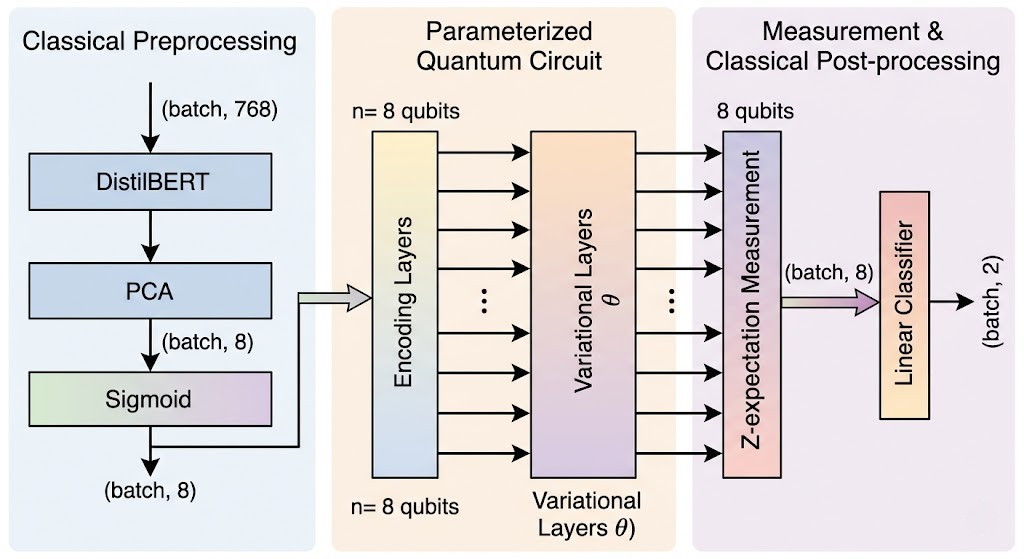
\includegraphics[width=0.85\textwidth]{FIGURE-Pipeline diagram.jpg}
\caption{Hybrid quantum-classical pipeline. Left: classical preprocessing (DistilBERT embedding, PCA reduction, sigmoid scaling) with data shapes at each stage. Center: parameterized quantum circuit with encoding and variational layers. Right: Z-expectation measurement feeding into a linear classifier for binary sentiment classification.}
\label{fig:pipeline}
\end{figure}

\textbf{Text Embedding.} We use a pre-trained DistilBERT~\cite{sanh2019} model (66M parameters, frozen) to extract 768-dimensional sentence embeddings from the [CLS] token representation for each text sample.

\textbf{Dimensionality Reduction.} Principal Component Analysis~\cite{sklearn} reduces the embedding from 768 to 8 dimensions, retaining approximately 36\% of total variance. The 8-dimensional output matches our circuit width (8 qubits for most encodings, 4 for Dense Angle). PCA is fitted exclusively on the training set; validation and test sets are transformed using the training-set projection, preventing data leakage.

\textbf{Sigmoid Scaling.} PCA outputs follow approximately $\mathcal{N}(0,1)$ distributions. However, angle-based quantum encodings expect inputs in $[0, \pi]$. We apply:
%
\begin{equation}
x_{\mathrm{scaled}} = \sigma(x_{\mathrm{PCA}}) \cdot \pi
\label{eq:sigmoid}
\end{equation}
%
This maps features to $[0, \pi]$, ensuring full Bloch sphere coverage: $R_y(0) = \ket{0}$ and $R_y(\pi) = \ket{1}$. Without this preprocessing, all encodings achieve only $\sim$52\% accuracy (majority-class prediction), compared to 60--70\% with sigmoid scaling (Section~\ref{sec:sigmoid}).

\textbf{Quantum Circuit.} Each encoding maps the 8 scaled features into a quantum state, followed by a shared variational ansatz with CZ entanglement (Section~\ref{sec:encodings}). We measure the Pauli-$Z$ expectation value on each qubit:
%
\begin{equation}
\langle Z_i \rangle = \langle \psi | Z_i | \psi \rangle = \sum_{j=0}^{2^n - 1} (-1)^{\mathrm{bit}(j,\, i)} \, |\alpha_j|^2
\label{eq:z_expectation}
\end{equation}
%
where $\alpha_j$ are the statevector amplitudes. This yields $n_{\mathrm{qubits}}$ real-valued outputs in $[-1, +1]$.

\textbf{Classifier.} A linear layer $W \in \mathbb{R}^{2 \times n_{\mathrm{qubits}}}$ with bias $b$ maps the Z-expectations to 2 logits for binary classification. The full model is trained end-to-end with cross-entropy loss via automatic differentiation on the statevector.

\subsection{Encoding Strategies}
\label{sec:encodings}

We evaluate four encoding strategies, all followed by the same variational ansatz with reps$=$1 (one entangling layer):

\textbf{Variational Ansatz (shared):}
\begin{equation}
\prod_{q} R_y(\theta_q) \prod_{q} R_z(\theta_q') \;\rightarrow\; \mathrm{CZ}_{\mathrm{linear}} \;\rightarrow\; \prod_{q} R_y(\theta_q'') \prod_{q} R_z(\theta_q''')
\end{equation}

Entanglement uses CZ (not CNOT/CX) gates in a linear nearest-neighbor topology.

\begin{figure}[t]
\centering
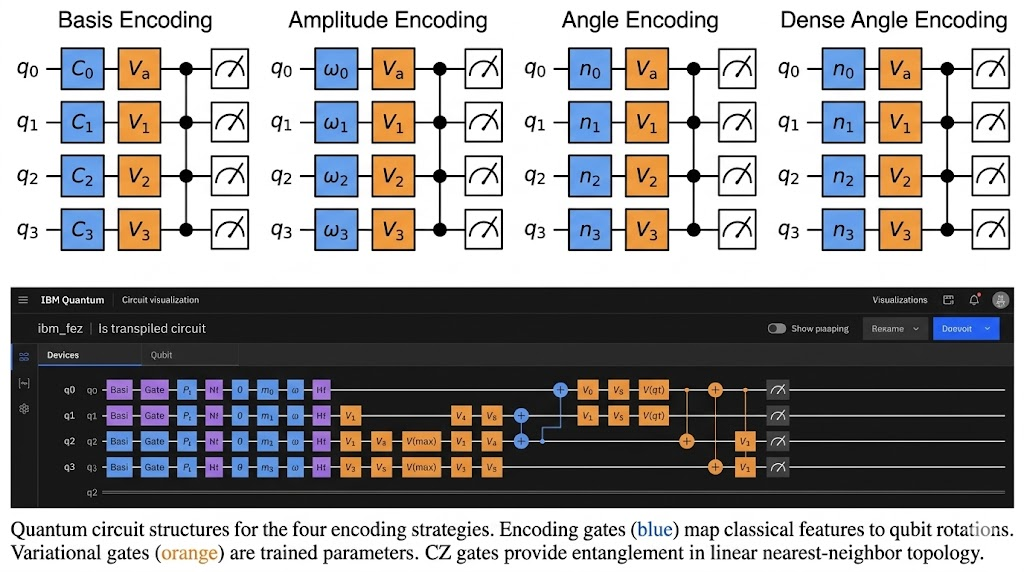
\includegraphics[width=0.85\textwidth]{FIGURE_4_circuit_diagrams.jpg}
\caption{Quantum circuit structures for the four encoding strategies. Encoding gates (blue) map classical features to qubit rotations. Variational gates (orange) are trained parameters. CZ gates provide entanglement in linear nearest-neighbor topology.}
\label{fig:circuits}
\end{figure}

\subsubsection{Angle Encoding (8 qubits, 50 parameters)}
Each PCA feature is encoded as a single $R_y$ rotation on a dedicated qubit:
\begin{equation}
\ket{0}_i \xrightarrow{R_y(\sigma(x_i) \cdot \pi)} \ket{\psi}_i \qquad \text{for } i = 0, 1, \ldots, 7
\end{equation}
One feature per qubit, no encoding-level entanglement. Transpiled depth on ibm\_fez: \textbf{19 gates}. Total: 32 quantum + 18 classical parameters.

\subsubsection{Dense Angle Encoding (4 qubits, 26 parameters)}
Two features per qubit using orthogonal rotation axes:
\begin{equation}
\ket{0}_i \xrightarrow{R_z(\sigma(x_{2i+1}) \cdot \pi) \; R_y(\sigma(x_{2i}) \cdot \pi)} \ket{\psi}_i \quad i = 0,\ldots,3
\end{equation}
Most qubit-efficient: 4 qubits, 3 CZ gates. Total: 16 quantum + 10 classical. Transpiled depth: \textbf{18 gates} (shallowest).

\subsubsection{IQP Encoding (8 qubits, 50 parameters)}
Instantaneous Quantum Polynomial encoding with pairwise feature interactions:
\begin{equation}
\ket{0}^{\otimes 8} \xrightarrow{H^{\otimes 8}} \xrightarrow{R_z(x_i)} \xrightarrow{R_{ZZ}(x_i \cdot x_{i+1})} \ket{\psi_{\mathrm{enc}}} \rightarrow \text{variational}
\end{equation}
The only encoding capturing inter-feature correlations. However, each $R_{ZZ}$ decomposes into CNOT--$R_z$--CNOT, and SWAP routing on ibm\_fez's heavy-hex topology further inflates the circuit. Transpiled depth: \textbf{101 gates} --- over $5\times$ deeper than any other encoding.

\subsubsection{Data Re-uploading Encoding (8 qubits, 50 parameters)}
Features re-encoded before each variational layer~\cite{perez2020}:
\begin{equation}
R_y(\mathbf{x}) \;\rightarrow\; [R_y(\theta) \cdot R_z(\theta) \cdot \mathrm{CZ}] \;\rightarrow\; \underbrace{R_y(\mathbf{x})}_{\text{re-upload}} \;\rightarrow\; [R_y(\theta) \cdot R_z(\theta)]
\end{equation}

\textbf{Important caveat:} This is a \emph{constrained} variant --- the second data upload is followed only by single-qubit rotations with \emph{no entangling CZ gates}, because all four encodings share the same ansatz (reps$=$1). Adding a second CZ layer would confound the encoding comparison. See Section~\ref{sec:reupload_discussion} for implications. Transpiled depth: \textbf{21 gates}.

\subsection{Gradient Variance Analysis}

To quantify trainability, we measure gradient variance at initialization following McClean et al.~\cite{mcclean2018barren}. For each encoding, we sample 100 random parameter initializations from $\mathcal{U}(0, 2\pi)$, compute the gradient of the loss via backpropagation, and report the mean gradient variance across all parameters. Higher variance indicates larger, more informative gradients.

\subsection{Training Configuration}

All models use identical hyperparameters: Adam optimizer~\cite{adam} ($\mathrm{lr}_q = 0.05$, $\mathrm{lr}_c = 0.001$), batch size 16, 30 epochs with early stopping (patience~10), ReduceLROnPlateau scheduler, identity initialization ($\theta = 0$), and 2000-sample subsets. Training uses PyTorch~\cite{pytorch} native statevector simulation, which is $3400\times$ faster than Qiskit's~\cite{qiskit} parameter-shift rule.

\subsection{Datasets}

\textbf{IMDb}~\cite{imdb}: 50{,}000 movie reviews for binary sentiment. We use a 2000-sample subset. \textbf{SST-2}~\cite{sst2}: Stanford Sentiment Treebank with binary labels, same subset protocol.

% ===================================================================
% 4. EXPERIMENTS AND RESULTS
% ===================================================================
\section{Experiments and Results}

\subsection{Multi-Seed Accuracy Comparison}

We train each encoding on IMDb with 5 random seeds (42, 123, 456, 789, 2024) and report mean accuracy $\pm$ standard deviation. SST-2 experiments use seed~42 for cross-dataset generalization.

\begin{figure}[t]
\centering
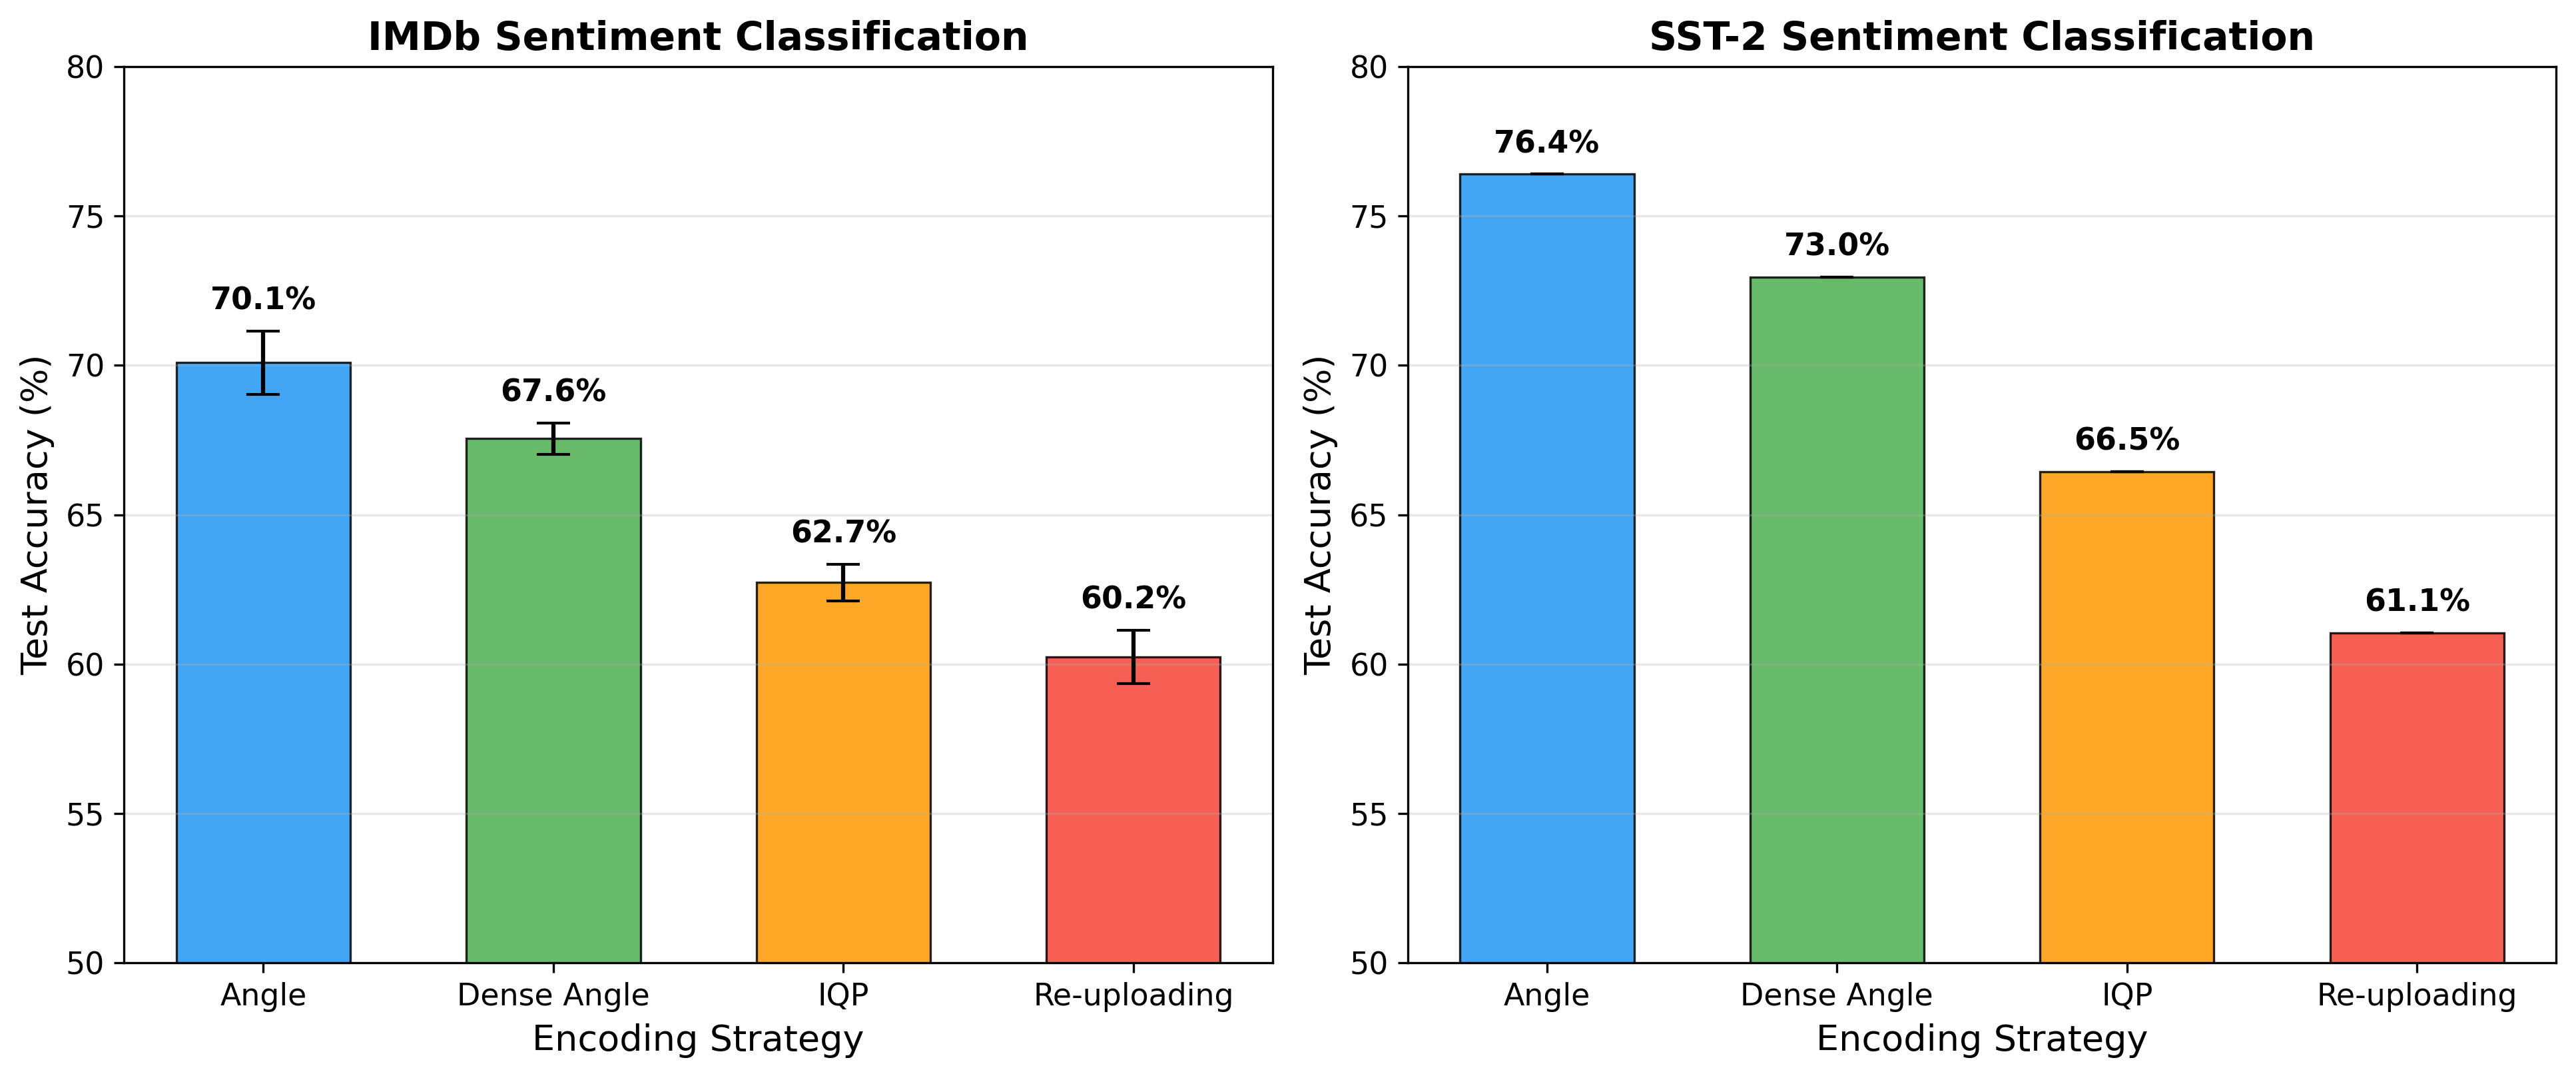
\includegraphics[width=0.85\textwidth]{fig4_multiseed_accuracy.png}
\caption{Test accuracy across random seeds. Error bars show standard deviation over 5 seeds (IMDb). The ranking Angle~$>$~Dense~$>$~IQP~$>$~Re-uploading is preserved across both datasets.}
\label{fig:multiseed}
\end{figure}

\begin{table}[t]
\centering
\caption{Encoding Comparison --- Simulator Results}
\label{tab:encoding_comparison}
\begin{tabular}{lccccc}
\toprule
Encoding & Qubits & Params & IMDb Acc (5 seeds) & SST-2 & Grad Var \\
\midrule
\textbf{Angle} & 8 & 50 & $\mathbf{70.1\% \pm 1.1\%}$ & $\mathbf{76.4\%}$ & 9.757 \\
Dense Angle & 4 & 26 & $67.6\% \pm 0.5\%$ & $73.0\%$ & 0.855 \\
IQP & 8 & 50 & $62.7\% \pm 0.6\%$ & $66.5\%$ & 0.899 \\
Re-uploading & 8 & 50 & $60.2\% \pm 0.9\%$ & $61.1\%$ & 9.098 \\
\midrule
\emph{Linear baseline} & \emph{---} & \emph{18} & \emph{72.2\%} & \emph{---} & \emph{---} \\
\bottomrule
\end{tabular}
\end{table}

\textbf{Key finding:} The encoding ranking (Angle $>$ Dense $>$ IQP $>$ Re-uploading) is \emph{identical} across all 5 seeds and both datasets, despite different text distributions and vocabulary. Not a single seed reverses any pairwise ranking. This strongly suggests encoding properties, rather than data-specific factors, dominate performance.

The linear classical baseline (72.2\%) outperforms all quantum models, consistent with our shallow circuits (reps$=$1). Our contribution is not a claim of quantum advantage but a systematic methodology for encoding selection.

\subsection{Gradient Variance--Accuracy Correlation}

\begin{figure}[t]
\centering
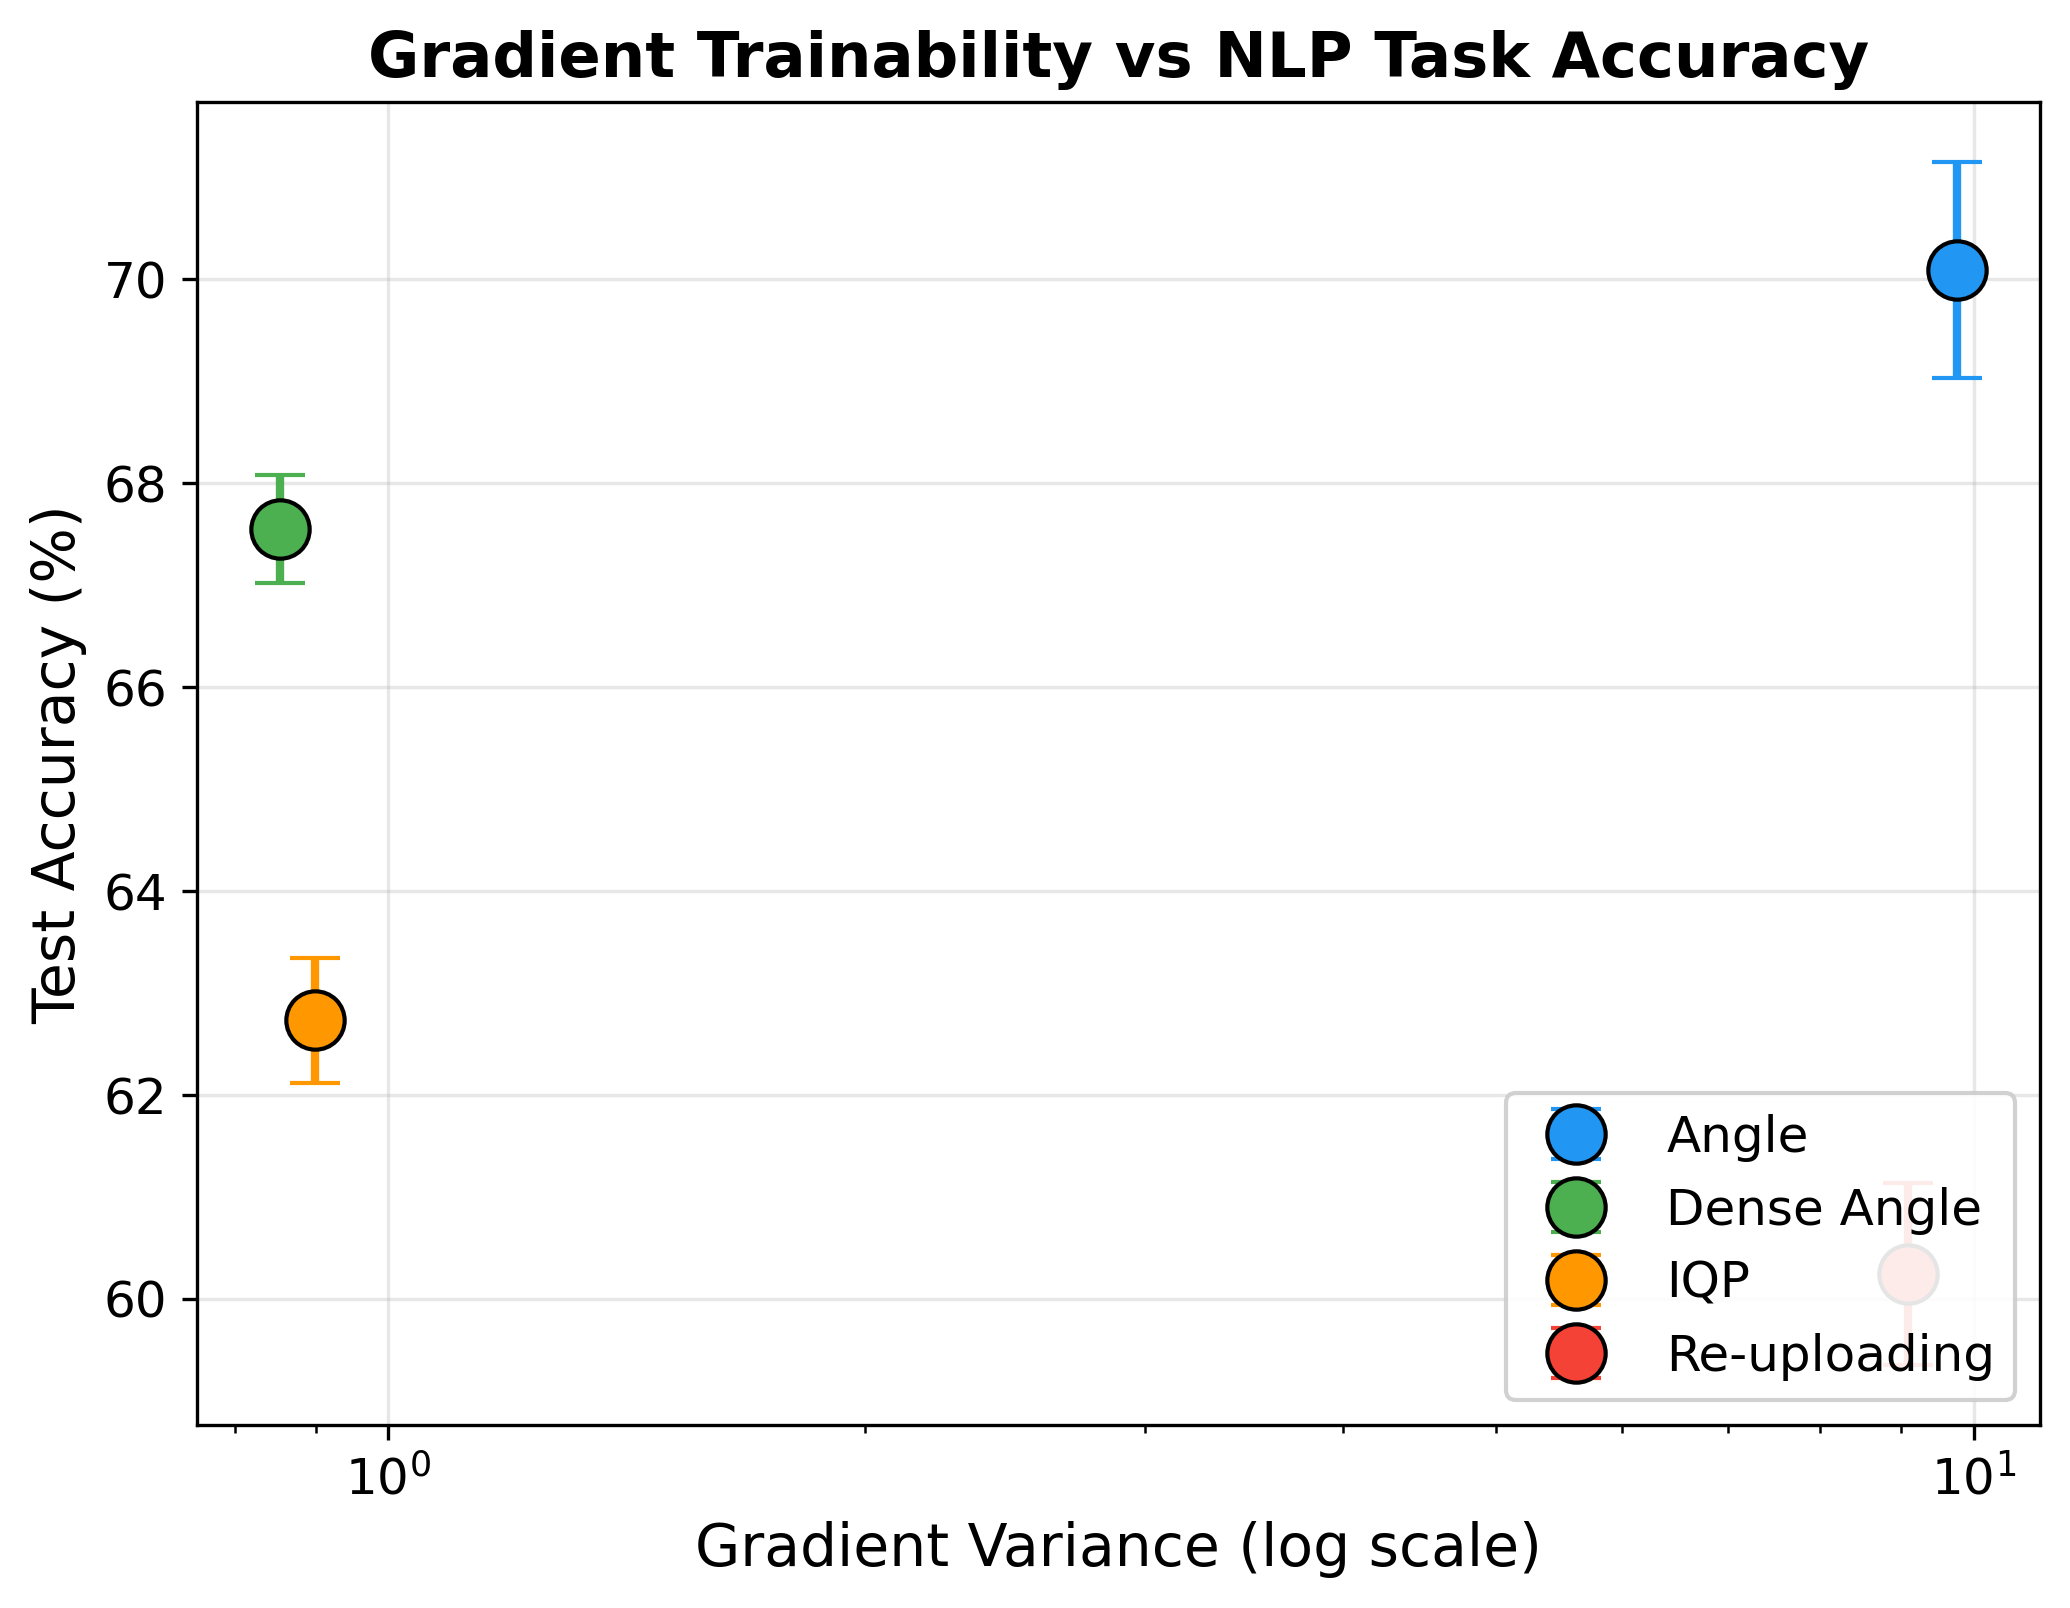
\includegraphics[width=0.85\textwidth]{fig1_variance_vs_accuracy.png}
\caption{Gradient variance at initialization vs.\ trained test accuracy. The relationship is non-monotonic: Angle (high variance, high accuracy) and Dense Angle (low variance, second-best accuracy) show that variance alone does not predict performance.}
\label{fig:variance_accuracy}
\end{figure}

\begin{figure}[t]
\centering
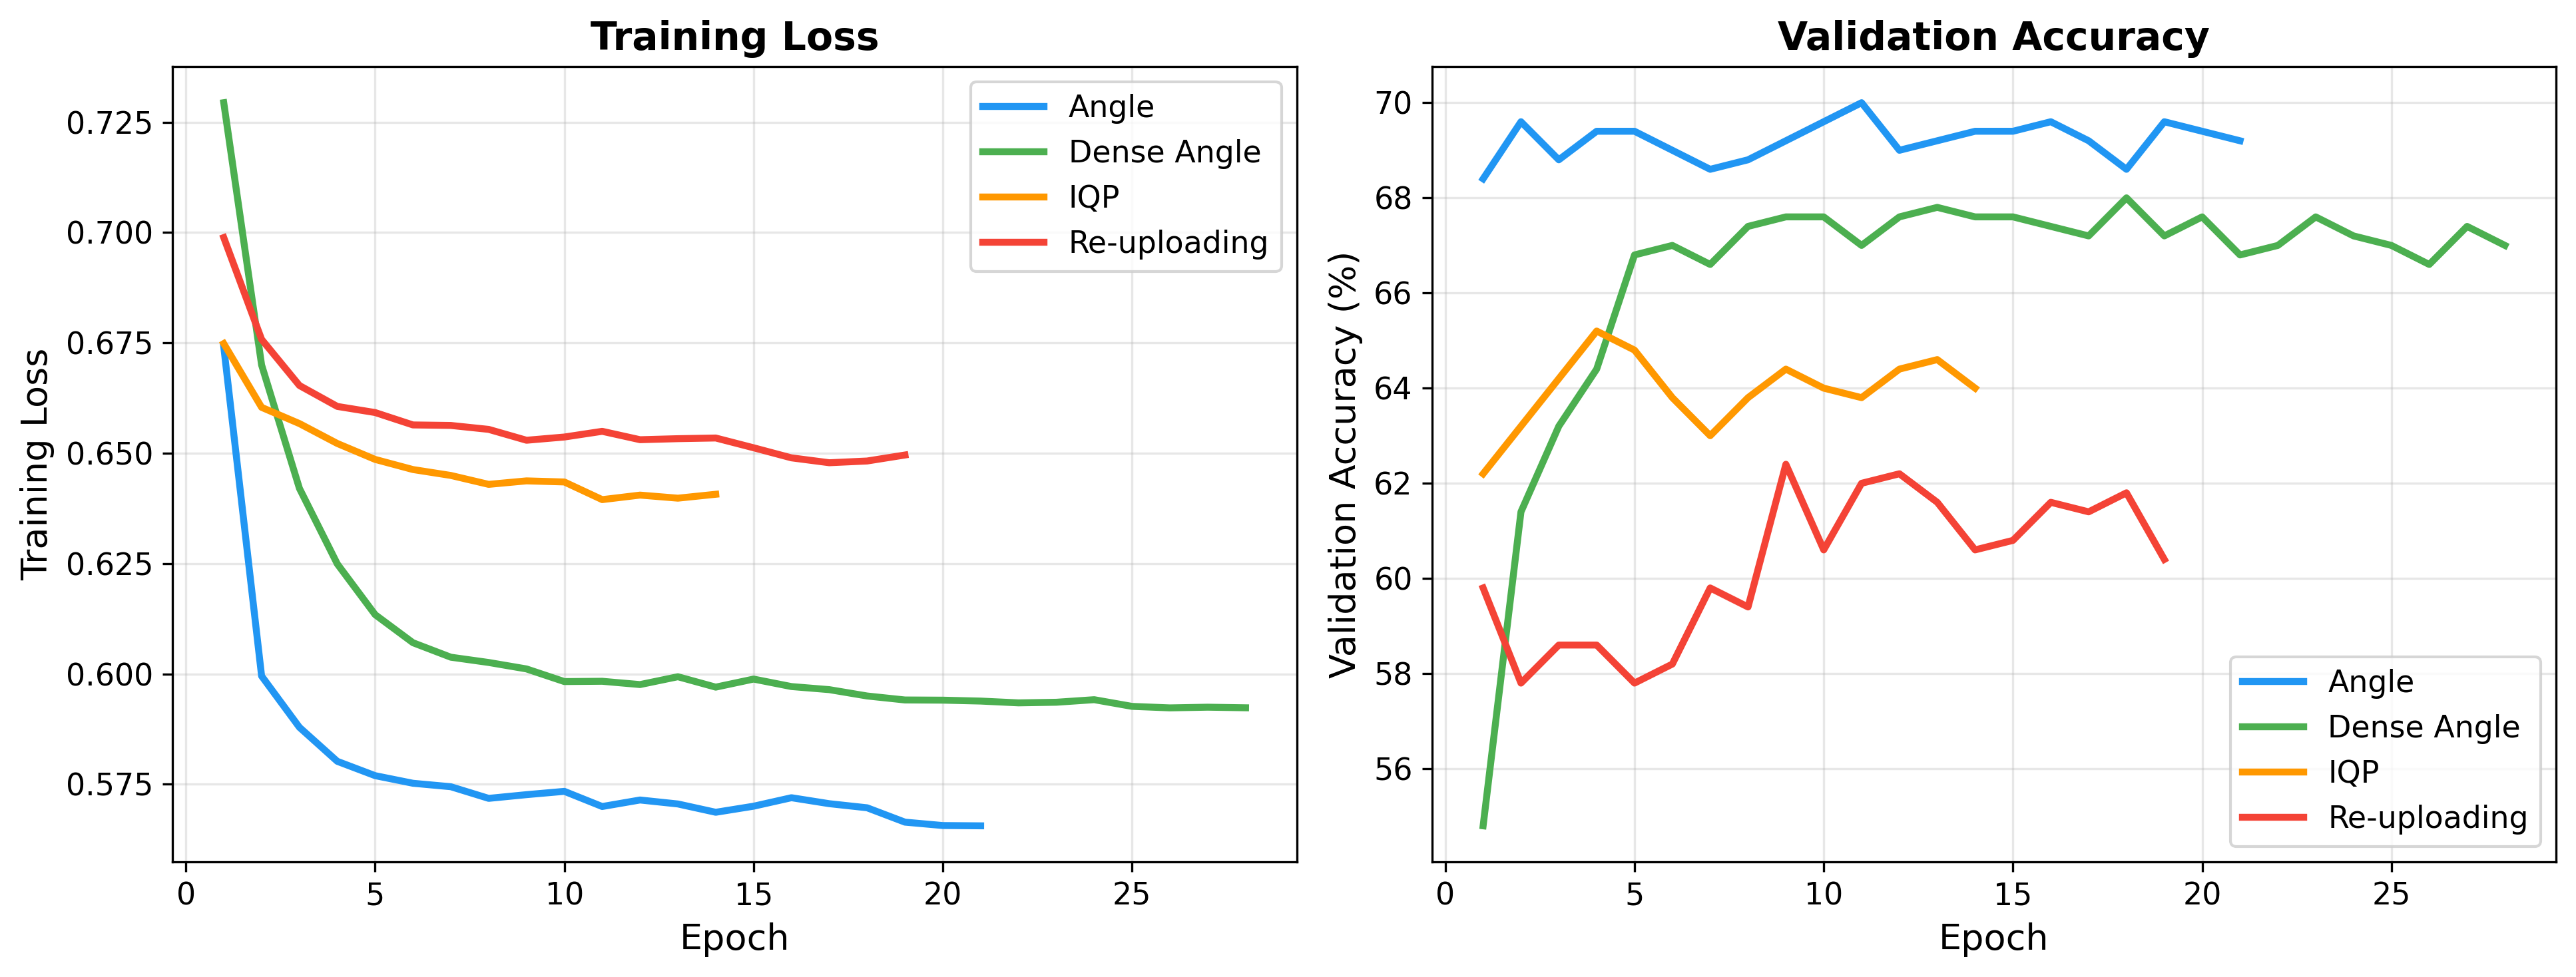
\includegraphics[width=0.85\textwidth]{fig2_training_curves.png}
\caption{Training dynamics of the four encoding strategies. Angle encoding converges fastest and achieves the lowest loss. IQP and Re-uploading show slower convergence.}
\label{fig:training_curves}
\end{figure}

\begin{table}[t]
\centering
\caption{Gradient Variance Analysis}
\label{tab:gradient}
\begin{tabular}{lcccc}
\toprule
Encoding & Mean Var & Mean $|\nabla|$ & Max Var & Accuracy \\
\midrule
Angle & 9.757 & 2.009 & 23.546 & 70.1\% \\
Re-uploading & 9.098 & 1.978 & 24.136 & 60.2\% \\
IQP & 0.899 & 0.582 & 2.687 & 62.7\% \\
Dense Angle & 0.855 & 0.578 & 1.817 & 67.6\% \\
\bottomrule
\end{tabular}
\end{table}

\textbf{Interpretation:} High variance facilitates optimization (Angle: $\mathrm{var}=9.76$, acc$=70.1\%$) but does not guarantee performance (Re-uploading: $\mathrm{var}=9.10$, acc$=60.2\%$). Conversely, low variance does not preclude strong performance: Dense Angle achieves $67.6\%$ with variance $0.855$, likely because its compact 4-qubit architecture has a smaller parameter space where even modest gradients suffice. Gradient variance is best understood as an \emph{informative diagnostic} rather than a strict predictor.

\subsection{Scaling Analysis}

\begin{figure}[t]
\centering
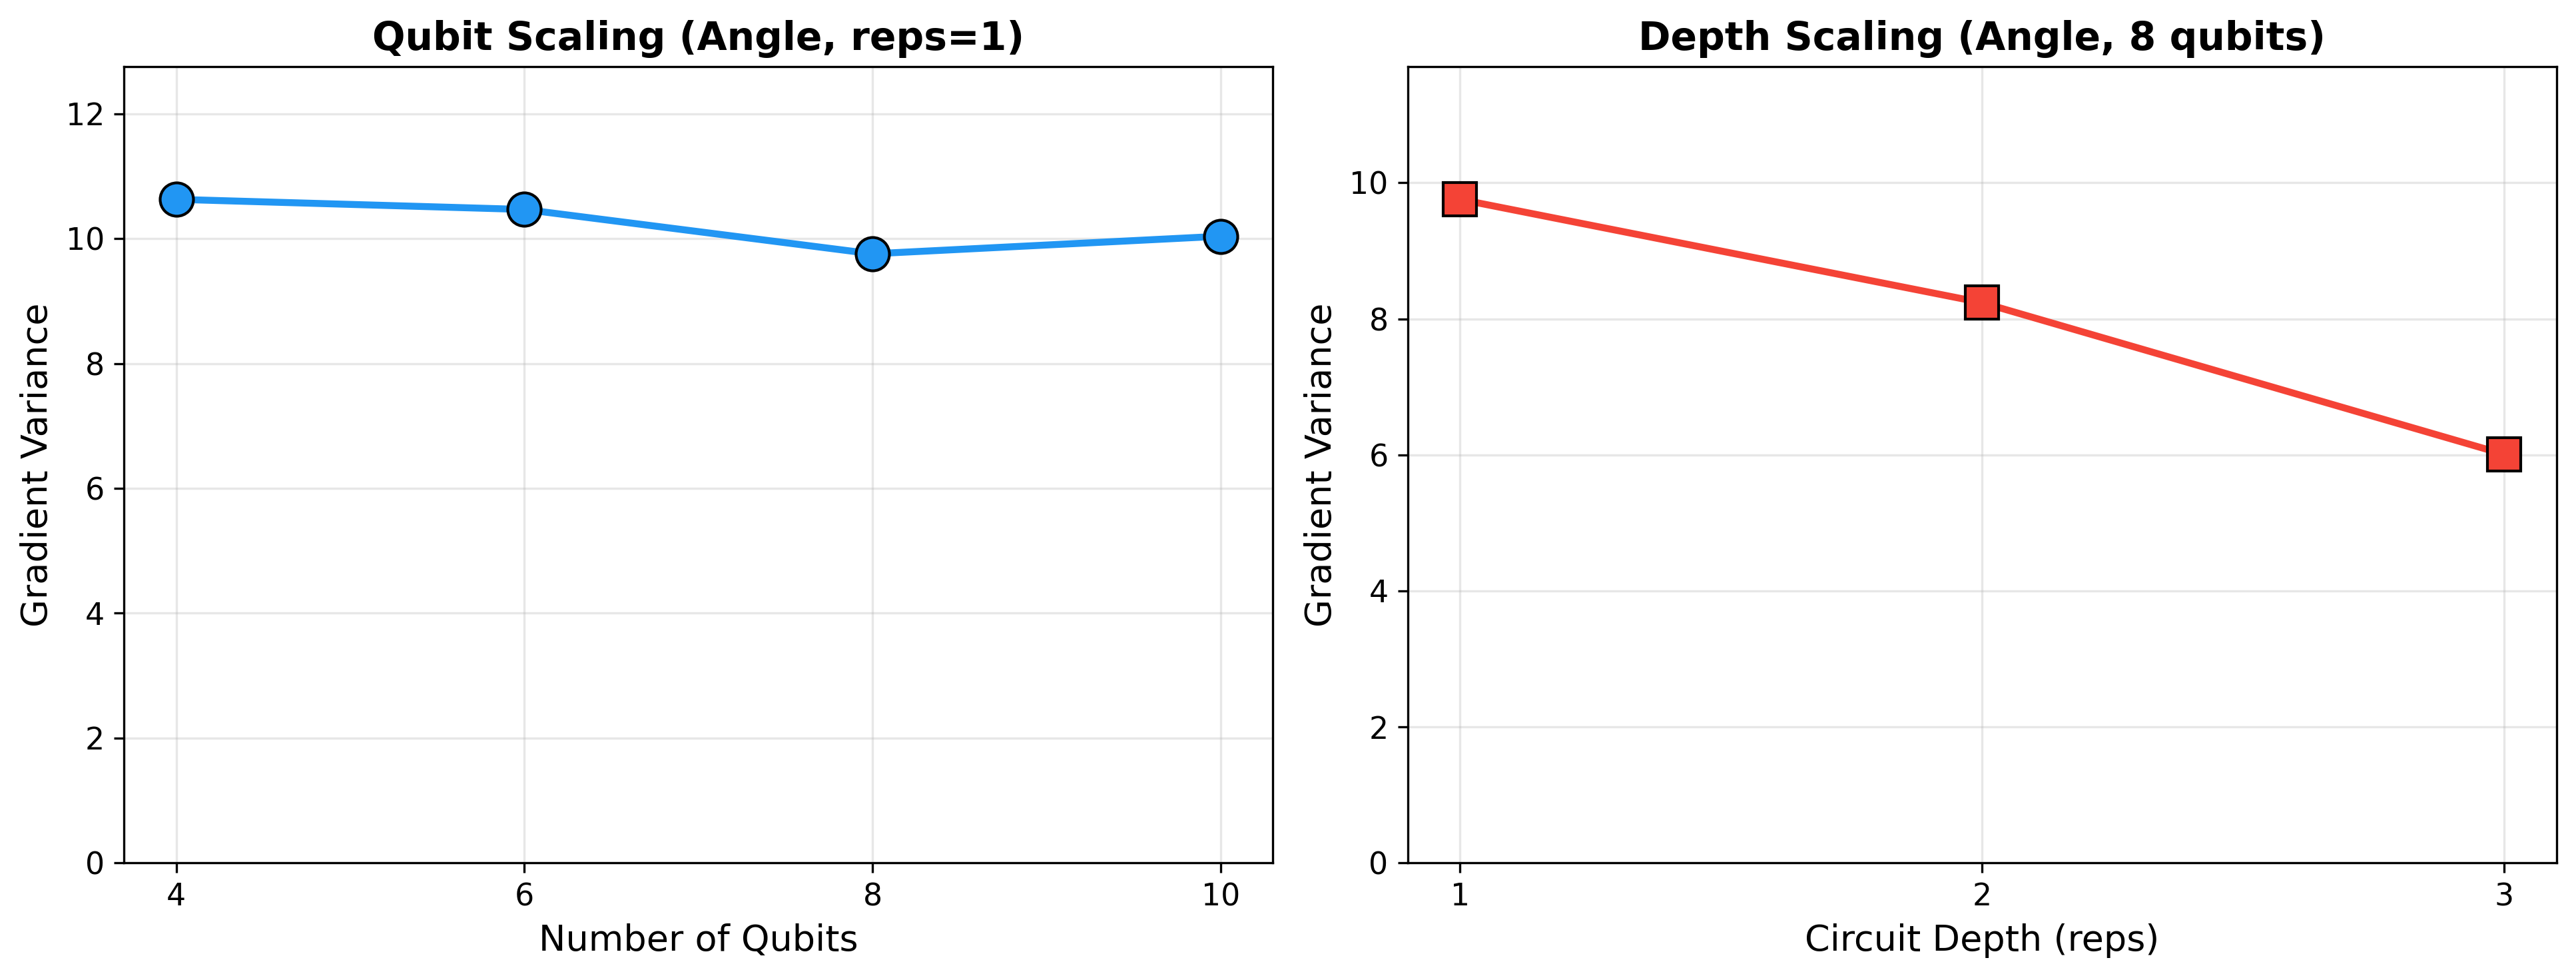
\includegraphics[width=0.85\textwidth]{fig3_scaling_analysis.png}
\caption{Gradient variance scaling with circuit width (left) and depth (right). Variance remains stable across 4--10 qubits, while increasing depth from reps$=$1 to reps$=$3 reduces variance by 38\%.}
\label{fig:scaling}
\end{figure}

In the 4--10 qubit range, gradient variance remains stable ($\sim$10), indicating no barren plateau onset. Increasing depth from reps$=$1 to reps$=$3 reduces variance by 38\% ($9.76 \rightarrow 6.01$), consistent with depth-induced barren plateaus, though gradients remain practically trainable.

\subsection{Sigmoid Scaling Effect}
\label{sec:sigmoid}

\begin{table}[t]
\centering
\caption{Impact of Sigmoid Preprocessing}
\label{tab:sigmoid}
\begin{tabular}{lcc}
\toprule
Preprocessing & Identity Init Acc & Random Init Acc \\
\midrule
None (raw PCA) & 51.6\% & 52.1\% \\
$\sigma(x) \cdot \pi$ & 68.8\% & 69.2\% \\
\midrule
\textbf{Improvement} & $\mathbf{+17.2}$~pp & $\mathbf{+17.1}$~pp \\
\bottomrule
\end{tabular}
\end{table}

Without sigmoid scaling, PCA outputs ($\sim \mathcal{N}(0,1)$) map to a narrow region of the Bloch sphere. Most values cluster between $-1$ and $+1$, keeping $R_y$ rotations near zero and qubit states close to $\ket{0}$. Sigmoid mapping transforms this distribution into $[0, \pi]$, spreading states across the full $\ket{0}$ to $\ket{1}$ arc. The improvement is consistent across initialization strategies, confirming it is an encoding-data alignment effect.

\subsection{IBM Quantum Hardware Validation}

We validate all four encodings on IBM's ibm\_fez quantum processor (156 qubits, Eagle~r3) using 10 test samples from the IMDb dataset. The primary metric is \textbf{simulator--QPU prediction fidelity}: how faithfully does noisy hardware reproduce the noise-free simulator's predictions?

\textbf{Test set design.} We use a \textbf{balanced test set} of 10 samples (5 negative / 5 positive, seed$=$42). This design is motivated by T1 amplitude damping: since T1 relaxation drives qubits toward $\ket{0}$, an all-negative set would confound hardware noise with correct label-0 prediction. Including label-1 samples tests whether circuits can maintain qubit states away from $\ket{0}$ --- the true measure of noise resilience.

\textbf{Parameter transfer.} Pre-trained variational parameters and classifier weights from PyTorch are transferred to Qiskit circuits with identical gate structure (critically using CZ, not CNOT). Transfer fidelity verified to 6 decimal places (Appendix~\ref{app:crossval}).

\textbf{QPU execution.} Qiskit Runtime Estimator~V2, transpiled with \texttt{optimization\_level=1}. Each sample requires $n_{\mathrm{qubits}}$ Pauli-$Z$ measurements packaged as PUBs. Total: 8 jobs, $\sim$5.5~min QPU time on IBM Quantum Open Plan.

\begin{figure}[t]
\centering
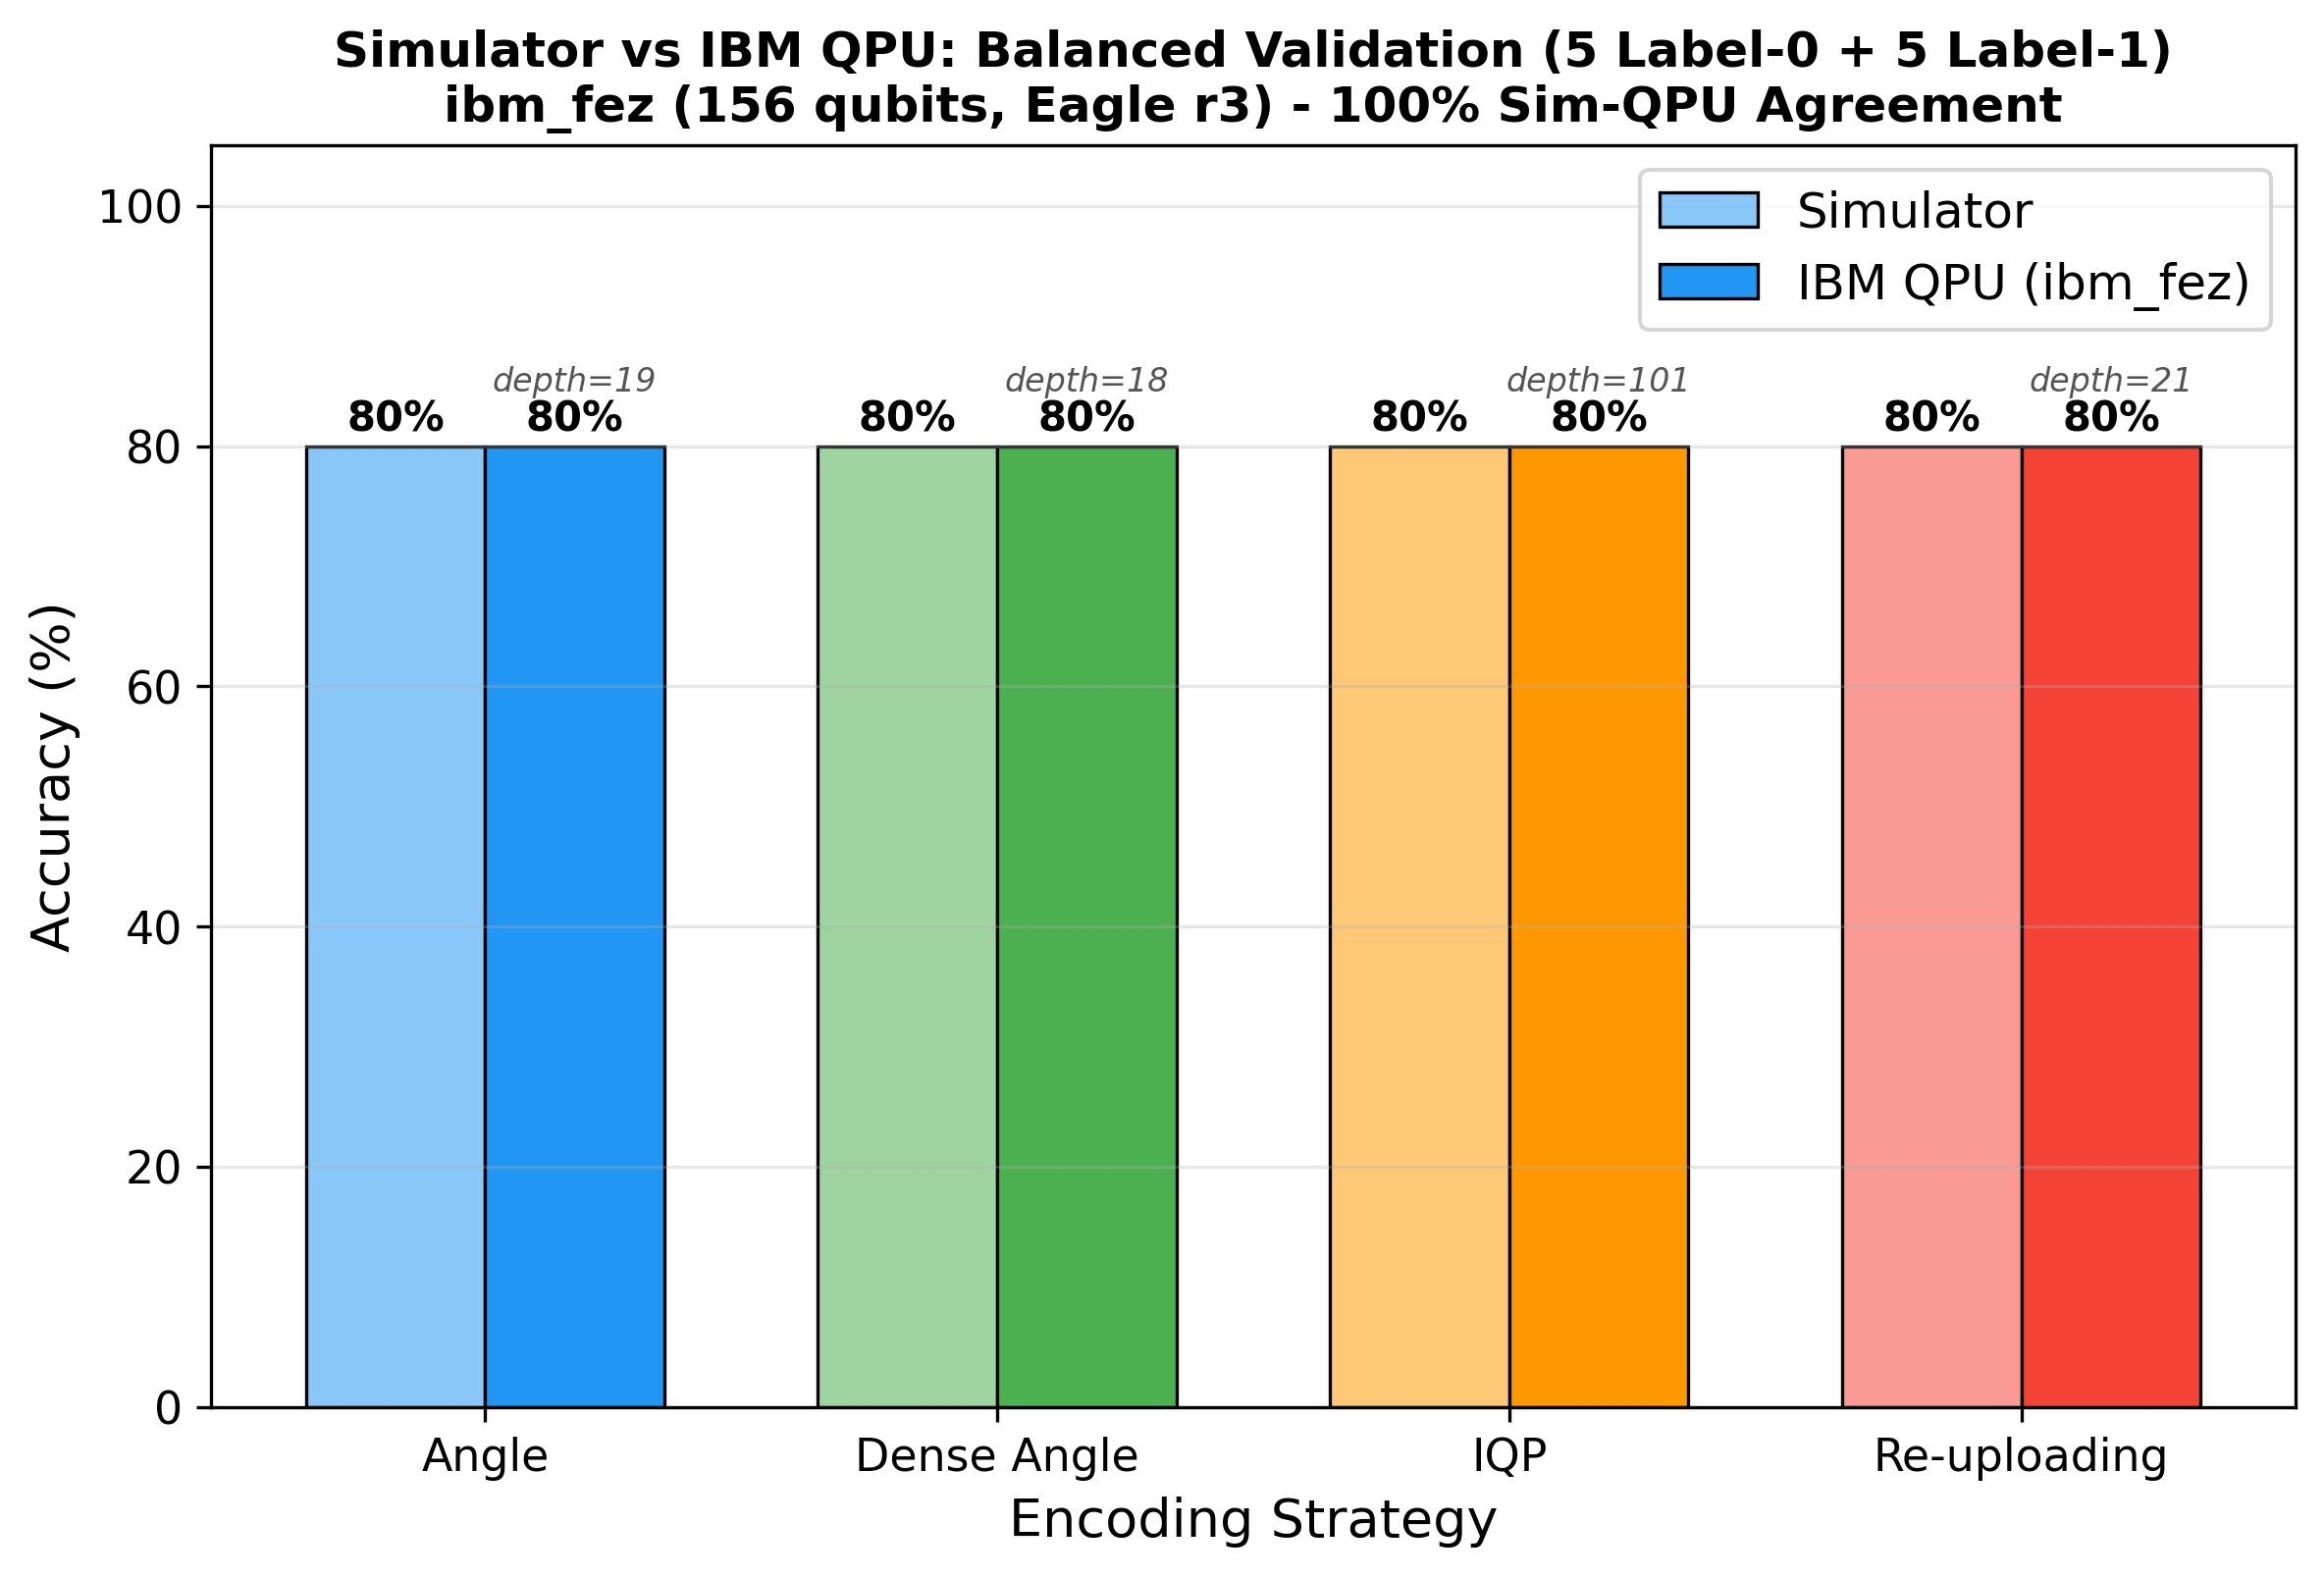
\includegraphics[width=0.85\textwidth]{fig5_ibm_qpu_comparison.png}
\caption{Simulator vs.\ IBM QPU accuracy for each encoding on ibm\_fez (156~qubits), balanced test set (5~label-0~+~5~label-1). Transpiled depth shown above bars. All encodings achieve 100\% Sim--QPU agreement --- no T1 bias detected.}
\label{fig:qpu}
\end{figure}

\begin{table}[t]
\centering
\caption{IBM QPU Balanced Validation (ibm\_fez, 10 samples: 5~label-0 + 5~label-1)}
\label{tab:qpu_balanced}
\begin{tabular}{lcccccc}
\toprule
Encoding & Sim & QPU & Agreement & L0 Agr & L1 Agr & Depth \\
\midrule
\textbf{Angle} & 80\% & 80\% & 10/10 & 5/5 & 5/5 & 19 \\
\textbf{Dense} & 80\% & 80\% & 10/10 & 5/5 & 5/5 & 18 \\
\textbf{IQP} & 80\% & 80\% & 10/10 & 5/5 & 5/5 & 101 \\
\textbf{Reupload} & 80\% & 80\% & 10/10 & 5/5 & 5/5 & 21 \\
\bottomrule
\end{tabular}
\end{table}

\textbf{Key observations:}

\begin{enumerate}
\item \textbf{Perfect simulator--QPU agreement across all encodings.} All four achieve 10/10 (100\%) prediction agreement with zero accuracy gap.

\item \textbf{No T1 relaxation bias detected.} Agreement is identical for label-0 (5/5) and label-1 (5/5) samples for every encoding. T1 amplitude damping, which drives qubits toward $\ket{0}$, would reduce label-1 fidelity if it were a confound. The symmetric agreement rules this out.

\item \textbf{IQP achieves perfect fidelity despite $5\times$ circuit depth.} The transpiled depth of 101 does not produce systematic degradation at this scale, though it remains a concern for larger deployments.

\item \textbf{All encodings correctly handle label-1 predictions on hardware.} Circuits maintain qubit states in the $\ket{1}$ direction against T1 relaxation for depths 18--101.
\end{enumerate}

\textbf{Sample-level analysis.} Every sample's prediction is identical between simulator and QPU. The two samples predicted incorrectly by all encodings (one label-0 error, one label-1 error) are model errors from the simulator faithfully reproduced on hardware, ruling out class-specific noise bias.

\begin{table}[t]
\centering
\caption{Angle Encoding --- Extended QPU Validation (ibm\_torino, 50 samples)}
\label{tab:qpu_torino}
\begin{tabular}{lcc}
\toprule
Metric & Simulator & QPU \\
\midrule
Pred$=$0 rate & 70.0\% (35/50) & 70.0\% (35/50) \\
Sim--QPU agreement & --- & 80\% (40/50) \\
Transpiled depth & --- & 42 \\
Execution time & 0.09s & 138.4s \\
\bottomrule
\end{tabular}
\end{table}

\begin{figure}[t]
\centering
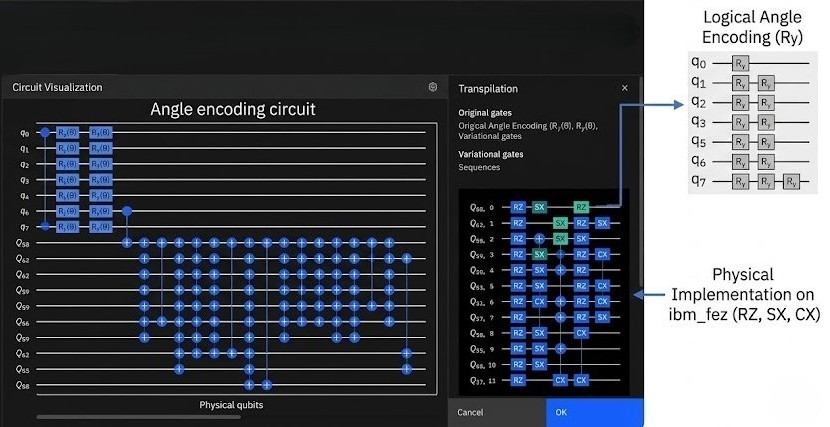
\includegraphics[width=0.85\textwidth]{IBM_circuit_screenshot.jpg}
\caption{IBM Quantum dashboard: transpiled Angle encoding circuit on ibm\_fez. Left: logical circuit with $R_y$ encoding and variational rotations on 8 qubits. Right: physical implementation after transpilation into the native gate set (RZ, SX, CX) with qubit routing on the heavy-hex topology. The transpiled depth of 19 gates reflects the shallow nature of Angle encoding.}
\label{fig:ibm_dashboard}
\end{figure}

% ===================================================================
% 5. DISCUSSION
% ===================================================================
\section{Discussion}

\subsection{Why Angle Encoding Wins}

Angle encoding's consistent top performance across both datasets and quantum hardware stems from: (1)~\emph{Simplicity} --- one $R_y$ per qubit, no encoding-level entanglement, minimal depth; (2)~\emph{High gradient variance} (9.76) enabling efficient optimization; (3)~\emph{Low transpiled depth} (19) minimizing noise accumulation on hardware.

\subsection{Re-uploading: Constrained Implementation}
\label{sec:reupload_discussion}

Our Re-uploading is a \emph{constrained variant}: the second data upload lacks entangling gates (to maintain equal ansatz depth). The original Perez-Salinas et al.~\cite{perez2020} formulation uses entanglement after each re-upload to generate multi-qubit Fourier terms. Without this, the re-uploaded features are processed purely locally, explaining the 10-point gap below Angle despite comparable gradient variance (9.10 vs.\ 9.76). Results should not be taken as evidence against re-uploading in general (see Limitation~\#8).

\subsection{Practical Encoding Selection Framework}

\begin{enumerate}
\item \textbf{Measure gradient variance as a diagnostic.} Low variance ($<1.0$) does not prevent training but signals careful tuning may be needed.
\item \textbf{Prefer shallow encodings.} Avoid decomposition-heavy gates ($R_{ZZ} \rightarrow$ CX--$R_z$--CX) for hardware deployment.
\item \textbf{Align input domains.} Sigmoid scaling is essential when inputs are not naturally in $[0, \pi]$.
\item \textbf{Validate on hardware early.} Simulator rankings may not hold on noisy hardware.
\end{enumerate}

\subsection{Limitations}

\begin{enumerate}
\item \textbf{Scale.} 8 qubits, classically simulable. May not extrapolate to 50+ qubits.
\item \textbf{PCA compression.} 768$\rightarrow$8 retains only $\sim$36\% variance. After compression, this is effectively 8-feature numeric classification.
\item \textbf{Sample size.} 2000-sample subsets for training.
\item \textbf{Single ansatz.} All encodings use the same variational layers.
\item \textbf{QPU sample size.} 10 samples per encoding (free-tier limits). Balanced design rules out T1 bias, but $N>100$ needed for confidence intervals.
\item \textbf{Sigmoid specificity.} Optimized for angle-based encodings; others may benefit from different scaling.
\item \textbf{Gradient methodology.} Variance measured at random $\mathcal{U}(0, 2\pi)$, but training uses identity init ($\theta=0$). Local variance analysis would strengthen the methodology.
\item \textbf{Re-uploading fairness.} Constrained variant lacks post-re-upload entanglement. Full evaluation requires reps$=$2.
\end{enumerate}

% ===================================================================
% 6. CONCLUSION
% ===================================================================
\section{Conclusion}

We presented a systematic comparison of four quantum data encoding strategies for NLP sentiment analysis, evaluated on IMDb and SST-2 with multi-seed validation and IBM quantum hardware testing. Key findings:

\begin{itemize}
\item \textbf{Encoding ranking is dataset-agnostic:} Angle $>$ Dense $>$ IQP $>$ Re-uploading, consistent across both benchmarks and all seeds.
\item \textbf{Gradient variance is informative but not sufficient:} High variance facilitates optimization but does not guarantee accuracy; low variance does not preclude strong performance in compact architectures.
\item \textbf{Input-domain alignment is critical:} Sigmoid scaling provides $+17$ points.
\item \textbf{Hardware validation confirms noise resilience:} Balanced QPU testing on ibm\_fez confirms 100\% simulator--QPU agreement for all encodings with zero T1 relaxation bias.
\end{itemize}

These results provide practitioners with a practical framework: measure gradient variance, prefer shallow circuits, align input domains, and validate on hardware. Future work should extend to larger qubit counts, explore encoding--ansatz co-optimization, and investigate task-specific encoding design.

% ===================================================================
% REFERENCES
% ===================================================================
\begin{thebibliography}{23}

\bibitem{cerezo2021vqa}
M.~Cerezo et~al., ``Variational quantum algorithms,'' \emph{Nature Reviews Physics}, vol.~3, no.~9, pp.~625--644, 2021.

\bibitem{bharti2022nisq}
K.~Bharti et~al., ``Noisy intermediate-scale quantum algorithms,'' \emph{Reviews of Modern Physics}, vol.~94, no.~1, p.~015004, 2022.

\bibitem{mcclean2018barren}
J.~R.~McClean et~al., ``Barren plateaus in quantum neural network training landscapes,'' \emph{Nature Communications}, vol.~9, p.~4812, 2018.

\bibitem{cerezo2021cost}
M.~Cerezo et~al., ``Cost function dependent barren plateaus in shallow parametrized quantum circuits,'' \emph{Nature Communications}, vol.~12, p.~1791, 2021.

\bibitem{schuld2021encoding}
M.~Schuld, R.~Sweke, and J.~J.~Meyer, ``Effect of data encoding on the expressive power of variational quantum machine-learning models,'' \emph{Physical Review A}, vol.~103, no.~3, p.~032430, 2021.

\bibitem{havlicek2019}
V.~Havl\'{i}\v{c}ek et~al., ``Supervised learning with quantum-enhanced feature spaces,'' \emph{Nature}, vol.~567, pp.~209--212, 2019.

\bibitem{mitarai2018}
K.~Mitarai et~al., ``Quantum circuit learning,'' \emph{Physical Review A}, vol.~98, no.~3, p.~032309, 2018.

\bibitem{larose2020}
R.~LaRose and B.~Coyle, ``Robust data encodings for quantum classifiers,'' \emph{Physical Review A}, vol.~102, no.~3, p.~032420, 2020.

\bibitem{shepherd2009}
D.~Shepherd and M.~J.~Bremner, ``Instantaneous quantum computation,'' \emph{Proc.\ Royal Society A}, vol.~465, pp.~1413--1439, 2009.

\bibitem{perez2020}
A.~Perez-Salinas et~al., ``Data re-uploading for a universal quantum classifier,'' \emph{Quantum}, vol.~4, p.~226, 2020.

\bibitem{imdb}
A.~L.~Maas et~al., ``Learning word vectors for sentiment analysis,'' in \emph{ACL}, 2011.

\bibitem{sst2}
R.~Socher et~al., ``Recursive deep models for semantic compositionality over a sentiment treebank,'' in \emph{EMNLP}, 2013.

\bibitem{tomal2025}
S.~R.~Tomal and S.~S.~Shafin, ``Quantum-enhanced attention mechanism in NLP,'' arXiv:2501.15630, 2025.

\bibitem{sasquatch}
E.~A.~Cherrat et~al., ``Learning with SASQuaTCh: Variational quantum transformers with kernel-based self-attention,'' arXiv:2403.14753, 2024.

\bibitem{setfit_pqc}
J.~Bowles et~al., ``SetFit-PQC: Few-shot quantum classification with SetFit,'' 2024.

\bibitem{hyqut}
Y.~Li et~al., ``HyQuT: Hybrid quantum transformer for language generation,'' arXiv:2511.10653, 2025.

\bibitem{gqhan}
C.~Yang et~al., ``GQHAN: Grover-inspired quantum hard attention network,'' 2024.

\bibitem{mele2024}
A.~A.~Mele et~al., ``Batched line search strategy for navigating through barren plateaus,'' \emph{Quantum}, 2024.

\bibitem{pytorch}
A.~Paszke et~al., ``PyTorch: An imperative style, high-performance deep learning library,'' in \emph{NeurIPS}, vol.~32, pp.~8026--8037, 2019.

\bibitem{qiskit}
A.~Javadi-Abhari et~al., ``Quantum computing with Qiskit,'' arXiv:2405.08810, 2024.

\bibitem{sanh2019}
V.~Sanh et~al., ``DistilBERT, a distilled version of BERT: smaller, faster, cheaper and lighter,'' arXiv:1910.01108, 2019.

\bibitem{adam}
D.~P.~Kingma and J.~Ba, ``Adam: A method for stochastic optimization,'' in \emph{ICLR}, 2015.

\bibitem{sklearn}
F.~Pedregosa et~al., ``Scikit-learn: Machine learning in Python,'' \emph{JMLR}, vol.~12, pp.~2825--2830, 2011.

\end{thebibliography}

% ===================================================================
% APPENDICES
% ===================================================================
\appendix

\section{Circuit Cross-Validation}
\label{app:crossval}

To ensure fidelity between PyTorch training and Qiskit QPU circuits, we built each circuit in both frameworks with identical parameters, computed Z-expectation values on the same input, and verified agreement to 6 decimal places.

\textbf{Critical bug discovered:} Initial Qiskit circuits used \texttt{EfficientSU2} with CX (CNOT) entanglement, while PyTorch uses CZ. All Qiskit circuits were replaced with manual builders using CZ. Without this correction, QPU results would have been invalid.

\section{Experimental Infrastructure}
\label{app:infra}

\begin{table}[h]
\centering
\begin{tabular}{ll}
\toprule
Component & Details \\
\midrule
Training GPU & NVIDIA RTX 4060 Laptop (CUDA 12.4) \\
Quantum sim & PyTorch-native statevector (CPU) \\
IBM QPU 1 & ibm\_torino, 133 qubits, Heron r2 \\
IBM QPU 2 & ibm\_fez, 156 qubits, Eagle r3 \\
QPU access & IBM Quantum Open Plan (10 min/month) \\
Primitive & Estimator V2 (Qiskit Runtime) \\
Total QPU time & $\sim$7 min across 9 jobs \\
Software & Python 3.13, PyTorch 2.6, Qiskit 2.3 \\
\bottomrule
\end{tabular}
\end{table}

\end{document}
